\documentclass[a4paper]{article}

\usepackage[english]{babel}
\usepackage[utf8x]{inputenc}
\usepackage{amsmath}
\usepackage{amsfonts}
\usepackage{graphicx}
\usepackage[colorinlistoftodos]{todonotes}

\title{CS 5785 -- Applied Machine Learning -- Lec.\ 7}
\author{Prof.\ Nathan Kallus, Cornell Tech\\Scribe: TBD}
\date{Sept.\ 14, 2017}

\begin{document}
\maketitle



\section{Singular Value Decomposition (SVD)}
First, a recap of \textit{eigenvectors} and \textit{eigenvalues}.
Given a matrix $\mathbf A$, a vector $x$ and a scalar $\lambda$ if it holds that ${\mathbf A}x=\lambda x$ then $x$ is an \textit{eigenvector} of ${\mathbf A}$ and $\lambda$ is the corresponding \textit{eigenvalue}.  In other words, if we multiply ${\mathbf A}$ by the vector $x$ we get back the same vector, scaled by some constant. 

Given ${\mathbf X}\in {\mathbb R}^{N\times p}$ we write its SVD as $\mathbf{X}=\mathbf{UD}\mathbf{V}^\top$. Where:
\begin{itemize}
\item ${\mathbf U}\in {\mathbb R}^{N\times p}$: Matrix of the left singular vectors.
\item ${\mathbf V}\in {\mathbb R}^{p\times p}$: Matrix of the right singular vectors.
\item ${\mathbf D}=diag\{d_1,d_2,\ldots, d_p\}\in {\mathbb R}^{p\times p}$, where for all the singular values it holds that $d_1\geq d_2\geq \ldots \geq d_p \geq 0$.
\end{itemize}
See Figure \ref{fig:SVDDiagram} for a visualization of this decomposition.

\begin{figure}
\centering
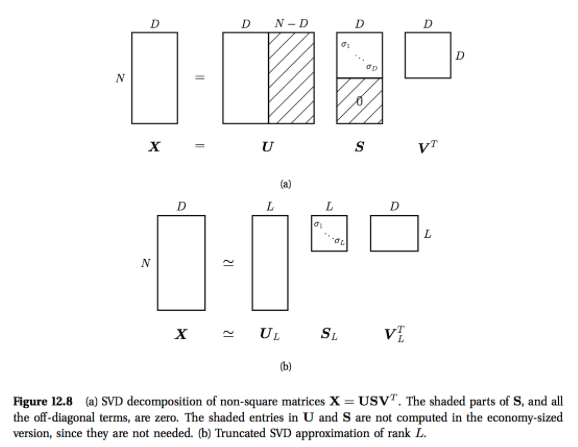
\includegraphics[width=1.0\textwidth]{SVD_diagram.png}
\caption{\label{fig:SVDDiagram} [Murphy] A diagram of SVD. Notice that in this example $\mathbf{D}$ is replaced by $\mathbf{S}$.}
\end{figure}
One thing that's very important to notice is that, if any single values from \textbf{D} equals to 0, some of our data (observation) is redundant. That way, we can say that the SVD can help us identify and minimize the existence of redundant data in our observations.

$\mathbf{U}$ and $\mathbf{V}$ both have orthogonal columns, so $\mathbf{U}^\top\mathbf{U}=\mathbf{I}$ and $\mathbf{V}^\top\mathbf{V}=\mathbf{I}$ where $\mathbf{I}$ is the identity matrix of size $p\times p$.

The SVD can help us extract useful information out of the original matrix $\mathbf{X}$.
Consider the matrix $\mathbf{X}^\top\mathbf{X}\in \mathbb{R}^{p \times p}$:
$$\mathbf{X}^\top\mathbf{X}=(\mathbf{UDV}^\top)^\top\mathbf{UDV}^\top=\mathbf{V} \mathbf{D}\mathbf{U}^\top\mathbf{UDV}^\top$$
D is diagonal, hence $\mathbf{D}^\top=\mathbf{D}$. Since $\mathbf{U}^\top\mathbf{U}=\mathbf{I}$ we get that:
$$\mathbf{X}^\top\mathbf{X}=\mathbf{VD}^2\mathbf{V}^\top$$
In other words, $\mathbf{VD}^2\mathbf{V}^\top$ is the eigendecomposition of $\mathbf{X}^\top\mathbf{X}$.  Notice that, by construction, the eigenvalues (i.e., entries of the diagonal matrix $\mathbf{D}^2$) are non-negative.  This means the matrix $\mathbf{X}^\top\mathbf{X}$ is \textit{positive semi-definite}.

We can also write the SVD as a sum of outer products: $$\mathbf{X}=\mathbf{UD}\mathbf{V}^\top=\sum_{j=1}^pd_ju_jv_j^\top$$
Where $u_j$ and $v_j$ are the  $j^{th}$ columns of $\mathbf{U}$ and $\mathbf{V}$, respectively. The sum in the above equation is a sum of rank $1$ matrices weighted by the scalars $d_j$.


\begin{figure}
\centering
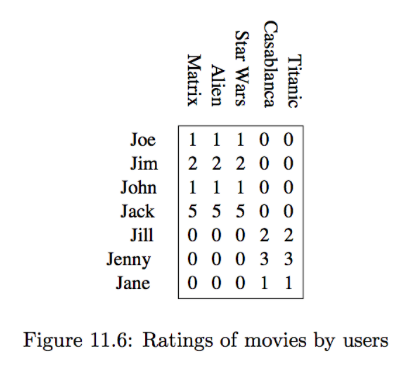
\includegraphics[width=1.0\textwidth]{people_by_movie_matrix.png}
\caption{\label{fig:PeopleByMovies}[Rajaraman, Leskovec \& Ullman]}
\end{figure}

Figure \ref{fig:PeopleByMovies} is an example of a data set of people's movie preferences represented by a matrix. Each row in this matrix represents the set of movie ratings of a given person, and each column represents a given movie's set of ratings.

\begin{figure}
\centering
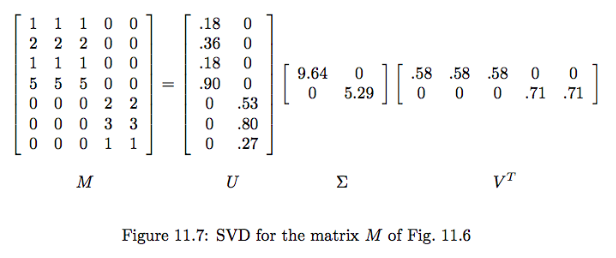
\includegraphics[width=1.0\textwidth]{movies_SVD.png}
\caption{\label{fig:SVDMovies}[Rajaraman, Leskovec \& Ullman]}
\end{figure}

Figure \ref{fig:SVDMovies} shows the SVD of matrix $\mathbf{M}$, the decomposition of matrix with all elements corrected to two significant digits. In this representation:

\begin{itemize}
\item we use economy-size decomposition to reduce extra zeros in singular value matrix, along with columns in $\mathbf{U}$,$\mathbf{V}$ that multiply those zeros, which reduces original dimension.
\item $\mathbf{U}$ connects people to concepts: Joe likes SciFi $(\mathbf{U}_{1,1}=.18)$ but not romance ($\mathbf{U}_{1,2}=0)$. 
\item $\mathbf{V}$ relates movies to concepts: \emph{The Matrix} (the movie) has $\mathbf{V}_{1,1}=.58$ and $\mathbf{V}_{1,2}=0$, which suggests that its genre is SciFi rather than romance.
\item $\Sigma$ is the strength of each concept. In this movie case, the strength of the SciFi concept is 12.4, while the strength
of the romance concept is 9.5, meaning the SciFi concept is stronger
because SciFi has more data supported information  on the movies of that genre and people who like it.

\end{itemize}

Given a vector of ratings from a new user Quincy: $q=[4,0,0,0,0]^\top$ (he only rated one movie, \emph{The Matrix}) we can get his genre preferences by calculating $q\mathbf{V}=[2.32,0]$. We can also try to predict his rating for the movies he hasn't seen by calculating $q\mathbf{VV}^\top=[1.35,1.35,1.35,0,0]$.

\begin{figure}
\centering
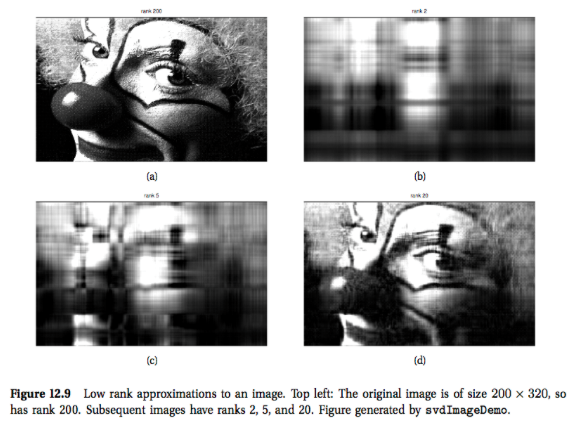
\includegraphics[width=1.0\textwidth]{clown_SVD.png}
\caption{\label{fig:SVDClown}[Murphy]}
\end{figure}

We can also use SVD to approximate pictures as seen in Figure \ref{fig:SVDClown}. The approximation is done by keeping only the leading entries (singular values) in $\mathbf{D}$, or equivalently, setting the singular values below some threshold to zero, and reconstructing the matrix. The more singular values we truncate, the coarser the approximation. In Figure \ref{fig:SVDClown} the top right image was reconstructed using only 2 singular values, the bottom left image used 5 and the bottom image used 20 (out of the original 200 nonzero singular values).


\section{Fisher's Linear Discriminant}
We now return to the discussion on linear discriminants by studying a method that allows us to project down the data, i.e., to perform \emph{dimensionality reduction}, in a supervised manner. It's important to notice that this method is not used for classification.

In many  applications we need to work with high dimensional data, which can be difficult to visualize.  Figure \ref{fig:coffee_beans_LDA} shows an example in which coffee bean odor is characterized by a 60 dimensional feature vector obtained using a gas sensor array.  Is it possible to find a lower dimensional representation of this data that preserves the separation between the classes? Fisher LDA provides one method for doing this. 

However, it is important to note that dimensionality reduction lowers data fidelity (unless a dimension is a linear variation of another). 

\begin{figure}
\centering
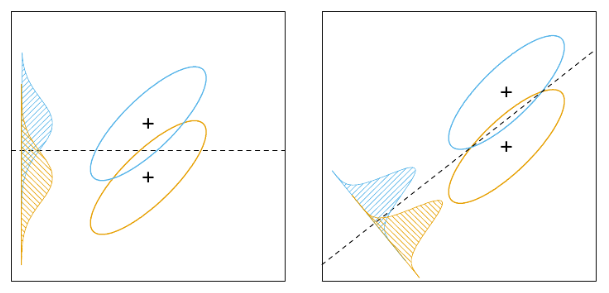
\includegraphics[width=1.0\textwidth]{projection_directions.png}
\caption{\label{fig:projection_directions}Fisher LDA seeks a projection direction (from 2D to 1D in this case) that provides good separation between the class densities.  In particular, it chooses the direction that maximizes between-class variance relative to within-class variance; such an example is shown on the right, compared to the example on the left that simply uses the the projection along the $x$ axis. [HTF Figure 4.9]}
\end{figure}


Consider the two class densities depicted in Fig.\ \ref{fig:projection_directions}.  Suppose we wanted to project this down to one dimension.  What is the best projection direction?  Fisher posed the problem as follows: 
\begin{quotation}
Find the linear combination $Z=a^\top X$ such that the \emph{between-class variance} is maximized relative to the \emph{within-class variance}.
\end{quotation}
This means that we are trying to find a projection that minimizes the overlap between the two densities. On our example, the image on the left shows the projection along the $x$-axis, i.e., using the vector $a=[1,0]^\top$.  That projection does keep the means separated, but there's still a troubling amount of overlap between the projected densities.  The example on the right shows a preferable projection direction, since the projected densities have considerably less overlap.

To make this precise, define the following quantities, where ${\hat \mu}_k$ and ${\hat \Sigma}$ are as defined in the previous lecture:
\begin{itemize}
\item ${\mathbf M}\in {\mathbb R}^{K\times p}$: matrix of class centroids (means).  It contains the $K$ sample means $\hat{\mu}_{k}$ (transposed) in its rows. The $k^{th}$ row is a vector of the $k^{th}$ class with the length of $p$ feature means. 
\item ${\mathbf W}\in {\mathbb R}^{p\times p}$: the within-class scatter matrix.  This is the same (up to a constant) as the pooled sample covariance $\hat{\Sigma}$ (pooling means ignoring the class).
\item ${\mathbf B}\in {\mathbb R}^{p\times p}$: the between-class scatter matrix.  It is equal (up to a constant) to the covariance matrix of the class centroids (i.e., rows of $\mathbf M$).
\end{itemize}
To compute $\mathbf B$ we take the mean of the class means, which we'll denote $\hat{\mu}$ (mean of the individuals mean vectors).  $\mathbf B$ is then given by
$$
{\mathbf B} = \sum_{k=1}^K (\hat{\mu}_k-\hat{\mu})(\hat{\mu}_k-\hat{\mu})^\top
$$
In the 2-class case, one can use $(\hat{\mu}_{1}-\hat{\mu}_{2})(\hat{\mu}_{1}-\hat{\mu}_{2})^\top$ instead of $\mathbf B$ without affecting the solution for $a$.

To answer the problem posed by Fisher, we maximize the following \emph{generalized Rayleigh quotient}, which is a ratio of two quadratic forms:
$$
\max_a \frac{a^\top {\mathbf B} a}{a^\top {\mathbf W} a}; a\in {\mathbb R}^{p\times 1}
$$
Equivalently we can solve the constrained maximization problem
$$
\max_a a^\top {\mathbf B} a \quad \text{subject to} \quad a^\top {\mathbf W} a=1
$$
This is a generalized eigenvalue problem with $a$ equal to the leading eigenvector\footnote{The leading eigenvector is the eigenvector corresponding to the largest eigenvalue.} of ${\mathbf W}^{-1}{\mathbf B}$. The vector $a$ is the best projection direction of the data from $p$ dimensions to $1$ dimension. Since we are looking for direction, the magnitude of $a$ is insignificant without loss of generality. In Figure \ref{fig:projection_directions}, $a$ is the direction of the vector on the right. We call the estimated $a$ vector the 1\textsuperscript{st} \emph{discriminant coordinate} or \emph{canonical variate} for the data, and we'll denote it $a_1$ here.  In this example we would stop with $a_1$, but in general, when $p>2$, we can solve for the next best projection direction $a_2$ by maximizing the Rayleigh quotient subject to the additional constraint that $a_2$ be orthogonal to $a_1$ in ${\mathbf W}$, i.e., $a_2^\top {\mathbf W} a_1=0$. For the next best projection, $a_3$, we assume that it is orthogonal to both $a_1$ and $a_2$ in $\mathbf W$, and so on.

To summarize, Fisher's LDA takes into account both the separation of the means and the spread (or ``scatter'') of the data when selecting the best projection direction.

\begin{figure}
\centering
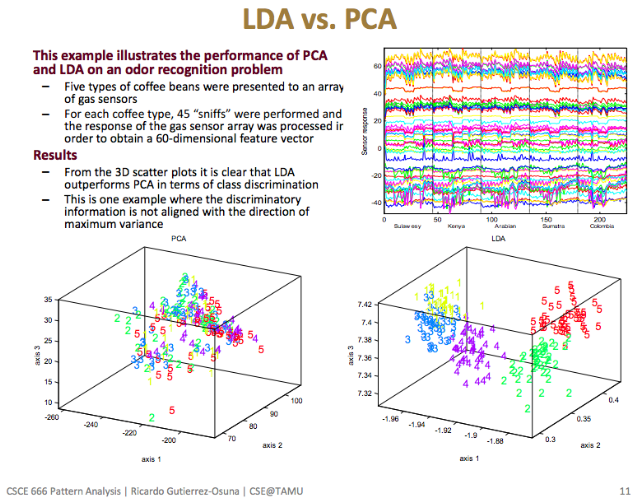
\includegraphics[width=1.0\textwidth]{coffee_beans_LDA.png}
\caption{\label{fig:coffee_beans_LDA} [Gutierrez-Osuna]}
\end{figure}

\section{Principal Components Analysis (a preview)}
Like Fisher's linear discriminant, PCA is a dimensionality reduction method that finds successive projection directions, but unlike LDA it is unsupervised.  PCA just computes one covariance matrix for all the data, while in Fisher's Linear Discriminant there are two covariance matrices (one of them is within-class and the other is between-class). The first \emph{principal axis} is the axis along which the data exhibits the greatest variance. (We'll cover how to compute this later in the semester.) In the example shown in Figure \ref{fig:projection_directions}, that would give us roughly the opposite of what Fisher LDA gives us, i.e., almost completely overlapping class densities.  This isn't meant as a criticism of PCA, since it's not the right tool to use when you have labelled classes, it's just intended as a point of comparison.  We'll still find PCA highly useful for dimensionality reduction in other problem settings.

In the example shown in Figure \ref{fig:coffee_beans_LDA} the plot on the lower right shows the dimensionality reduction from 60 to 3 as calculated by Fisher LDA and on the left by PCA. Fisher LDA clearly provides superior class separation.  The three discriminant coordinates it finds are all linear transformations of the raw 60-dimensional feature vectors (of the form $Z=a^\top X$), i.e., each coordinate represents some linear combination of measurements from different nodes in the gas sensor array. To get an intuitive interpretation of these three axes (e.g., sweetness, sourness, bitterness) we'd need to ask a barista.



\end{document}
